\documentclass[12pt]{article}

\usepackage{graphicx}
\usepackage{paralist}
\usepackage{amsfonts}
\usepackage{amsmath}
\usepackage{hhline}
\usepackage{booktabs}
\usepackage{multirow}
\usepackage{multicol}
\usepackage{url}
\usepackage{hyperref}

\oddsidemargin -10mm
\evensidemargin -10mm
\textwidth 160mm
\textheight 200mm
\renewcommand\baselinestretch{1.0}

\pagestyle {plain}
\pagenumbering{arabic}

\newcounter{stepnum}

%% Comments

\usepackage{color}

\newif\ifcomments\commentstrue

\ifcomments
\newcommand{\authornote}[3]{\textcolor{#1}{[#3 ---#2]}}
\newcommand{\todo}[1]{\textcolor{red}{[TODO: #1]}}
\else
\newcommand{\authornote}[3]{}
\newcommand{\todo}[1]{}
\fi

\newcommand{\wss}[1]{\authornote{blue}{SS}{#1}}

\title{Assignment 4, Specification}
\author{SFWR ENG 2AA4, COMP SCI 2ME3}

\begin {document}

\maketitle
This Module Interface Specification (MIS) document contains modules, types and methods for implementing 2048. The game begins with a board that consist of two randomly generated tiles of values 2 or 4. The user can move the tiles up, down, left or right. When shifted, adjacent tiles with the same values will be combined together. Note that each tile, can only be combined once per move. Tiles with similar values will remain in their current position and will not be combined. If the adjacent value is zero, the tile will continue to move across the board, until it hits the edge of the board or a tile with a different value. The player loses when the  all tiles cannot be moved anymore. On the other hand, the player wins when they have combined enough tiles to create a tile with a value of 2048. The game can be launched and play by typing \verb|make expt| in terminal. Note. use "a", "w", "s", and "d" to control tiles.

\begin{center}
  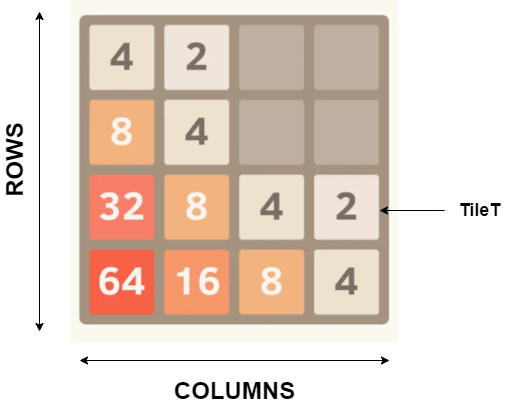
\includegraphics[width=0.6\textwidth]{2048_board_labelled.png}

  The 2048 board image above is from https://apps.apple.com/ca/app/2048-by-gabriele-cirulli/id868076805.
\end{center}

\newpage

\section{Overview of the design}

This design applies Module View Specification (MVC) design pattern.The MVC components are \textit{Controller} (controller module), \textit{BoardT} (model module), and \textit{UserInterface} (view module). \textit{BoardT} uses Move \textit{Move} to merge tiles in a given direction. While, \textit{Direction} provides enumerated types for the tile movements and is used by \textit{Move}.

\noindent A UML diagram is provided below to vvisualize the software architecture.

\begin{center}
  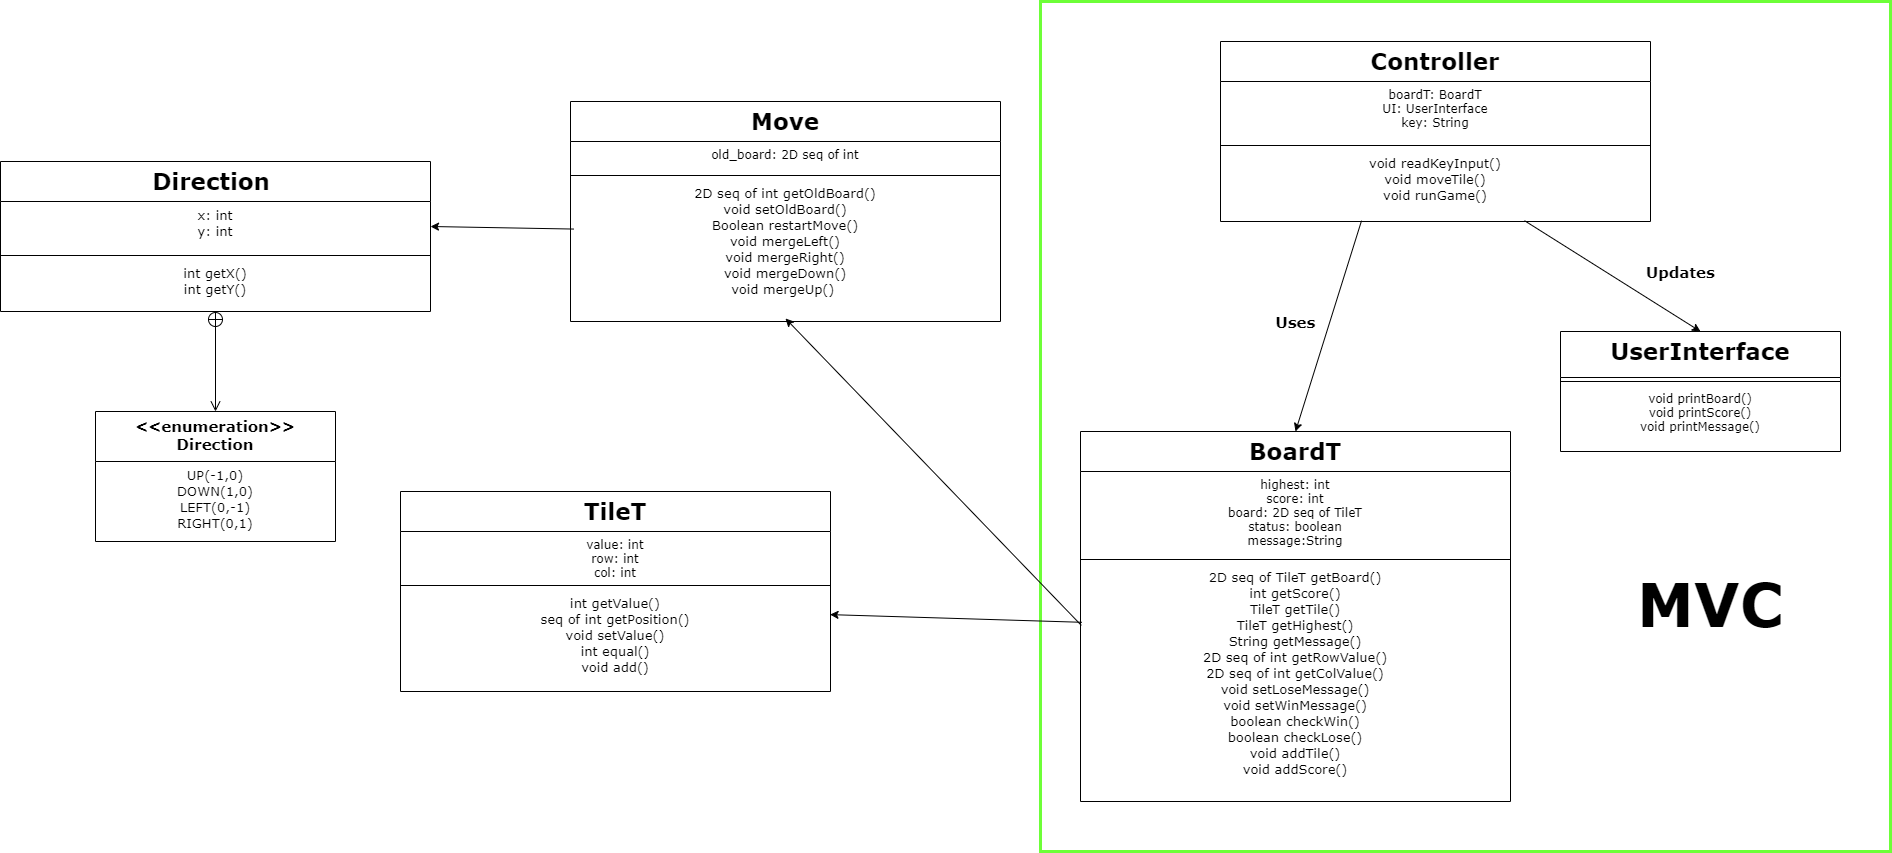
\includegraphics[width=1\textwidth]{UML.png}
\end{center}

\medskip

The MVC design pattern seprates the model, user interface, and the controls into three components. For this game, the MVC design pattern is implemented in the following way: the module \textit{BoardT} stores the state and status of the board. The \textit{Userinterface} is the view portion of MVC. It displays the state of the board using ASCII graphics. The controller uses the state of \textit{BoardT} and is able to manipulate it. It also updates the UserInterface.

\newpage

\subsection*{Likely Changes my design considers:}

\begin{itemize}
  \item Data structure, array, used to store the game board.
  \item The game halts, when 2048 has been reached.
  
\end{itemize}

\newpage


\section* {Board Module}

\subsection*{Template Module}

BoardT

\subsection* {Uses}

TileT

\subsection* {Syntax}

\subsubsection* {Exported Constants}

Size = 4 //Size of the board 4 x 4

\subsubsection* {Exported Types}

BoardT = ?

\subsubsection* {Exported Access Programs}

\begin{tabular}{| l | l | l | p{5cm} |}
  \hline
  \textbf{Routine name} & \textbf{In} & \textbf{Out} & \textbf{Exceptions}\\
  \hline
  new BoardT & & BoardT & \\
  \hline
  getBoard & & seq of (seq [4] of TileT) & ~\\
  \hline
  getScore & & $\mathbb{N}$ & ~\\
  \hline
  getTile & $\mathbb{N}$, $\mathbb{N}$ & TileT & ~\\
  \hline
  getHighest & & TileT & ~\\
  \hline
  getMessage & & String & ~\\
  \hline
  getRowValue & $\mathbb{N}$ & seq [4] of $\mathbb{N}$ & ~\\
  \hline
  getColValue & $\mathbb{N}$ & seq [4] of $\mathbb{N}$ & ~\\
  \hline
  setLoseMessage & & & ~\\
  \hline
  setWinMessage & & & ~\\
  \hline
  checkWin & & $\mathbb{B}$ & ~\\
  \hline
  checkLose & & $\mathbb{B}$ & ~\\
  \hline
  addTile & & & ~\\
  \hline
  addScore & $\mathbb{N}$ & & ~\\
  \hline
  
\end{tabular}

\subsection* {Semantics}

\subsubsection* {State Variables}
$highest : \mathbb{N}$\\   
$score : \mathbb{N}$\\
$board$ : seq of (seq [4] of TileT)\\
$message$ : String\\

\subsubsection* {State Invariant}

None

\subsubsection* {Assumptions}
\begin{itemize}
  \item The constructor BoardT is called for each object instance and before any other access routine for that object.
  \item Assume a random function that generates a random value between 0 and 1.
\end{itemize}

\subsubsection* {Access Routine Semantics}

\noindent new BoardT():
\begin{itemize}
\item transition: \\
     board $:=$
     $\langle \begin{array}{c}
      \langle \mbox{TileT()}_0, ... ... ,\mbox{TileT()}_3 \rangle\\
      \langle \mbox{TileT()}_0, ... ... ,\mbox{TileT()}_3 \rangle\\
      \langle \mbox{TileT()}_0, ... ... ,\mbox{TileT()}_3 \rangle\\
      \langle \mbox{TileT()}_0, ... ... ,\mbox{TileT()}_3 \rangle\\
      \end{array} \rangle $ \\ 
      where the value of any two random tiles is $2$ or $4$ and the rest are $0$,\\
      highest, score $=$  0, 0
\item output: $out := \mathit{self}$
\item exception: none
\end{itemize}

\noindent getBoard():
\begin{itemize}
\item output: $out := board$
\item exception: none
\end{itemize}

\noindent getScore():
\begin{itemize}
\item output: $out := score$
\item exception: none
\end{itemize}

\noindent getTile(row, col):
\begin{itemize}
\item output: $out := board[row][col]$ 
\item exception: none
\end{itemize}

\noindent getHighest():
\begin{itemize}
\item output: $out := (\exists x : TileT | x \in board \land \forall(y : TileT | y \in board \land x >= y : x))$ 
\item exception: none
\end{itemize}

\noindent getMessage():
\begin{itemize}
\item output: $out := message$ 
\item exception: none
\end{itemize}

\noindent getRowValue(row):
\begin{itemize}
\item output: $out := [i : \mathbb{N} | i \in [0.. |board|-1] : board[row][i]]$ 
\item exception: none
\end{itemize}

\noindent getColValue(col):
\begin{itemize}
\item output: $out := [i : \mathbb{N} | i \in [0.. |board|-1] : board[i][col]]$ 
\item exception: none
\end{itemize}

\noindent setLoseMessage():
\begin{itemize}
\item transition:\\ 
$message :=$ A message to represent the player lost
\item exception: none
\end{itemize}

\noindent setWinMessage():
\begin{itemize}
\item transition:\\ 
$message :=$ A message to represent the player won
\item exception: none
\end{itemize}

\noindent addTile():
\begin{itemize}
\item transition: \\
 $val = generateRandomTile \land pos = generateRandomPosition \\
 \implies board[pos[0][pos[1]].setValue(val) $
\item exception: none
\end{itemize}

\noindent addScore(points):
\begin{itemize}
\item transition:\\
$score := score + points$
\item exception: none
\end{itemize}

\noindent checkWin():
\begin{itemize}
\item output := $\exists(t : TileT | t \in board : t.getValue() = 2048)$
\item exception: none
\end{itemize}

\noindent checkLose():
\begin{itemize}
\item output := $\forall(i, j : \mathbb{N}\ |\ i, j \in [0..|board|-1] : board[i][j].getValue() \neq board[i][j+1] \land board[i+1][j].getValue() \neq board[i+1][j]\ \land board[i][j].getValue() \neq 0\ \land board[i][j].getValue() \neq 2048)$
\item exception: none
\end{itemize}


\subsection*{Local Functions}

\noindent generateRandomTile: $\mathbb{N}$\\
\noindent $\mbox{generateRandomTile()} \equiv Math.random() < 0.9 \implies 2  | True \implies 4$

~\\

\noindent generateRandomPosition: seq of $\mathbb{N}$\\
\noindent $\mbox{generateRandomPosition()} \equiv \exists (i,j : \mathbb{N}\ |\ board[i][j] \neq 0 : [i,j])$; 
\newpage




\newpage

\section* {TileT Module}

\subsection*{Template Module}
TileT

\subsection* {Uses}

None

\subsection* {Syntax}

\subsubsection* {Exported Constants}

None

\subsubsection* {Exported Types}

TileT = ?

\subsubsection* {Exported Access Programs}

\begin{tabular}{| l | l | l | p{5cm} |}
  \hline
  \textbf{Routine name} & \textbf{In} & \textbf{Out} & \textbf{Exceptions}\\
  \hline
  new TileT & & TileT & \\
  \hline
  getValue & & $\mathbb{N}$ & ~\\
  \hline
  getPosition & & seq of $\mathbb{N}$ & ~\\
  \hline
  setValue & $\mathbb{N}$ & & ~\\
  \hline
  equal & TileT & $\mathbb{N}$ & ~\\
  \hline
  add & & & ~\\
  \hline
  
\end{tabular}

\subsection* {Semantics}

\subsubsection* {State Variables}
$value : \mathbb{N}$\\   
$row : \mathbb{N}$\\
$col : \mathbb{N}$\\

\subsubsection* {State Invariant}

None

\subsubsection* {Assumptions}

None

\subsubsection* {Access Routine Semantics}

\noindent new TileT(val, row, col):
\begin{itemize}
\item transition: $value, row, col := val, row, col$
\item output: $out := \mbox{self}$
\item exception: none
\end{itemize}

\noindent getValue():
\begin{itemize}
\item output: $out := value$
\item exception: none
\end{itemize}

\noindent getPosition():
\begin{itemize}
\item output: $out := [row, col]$
\item exception: none
\end{itemize}

\noindent setValue(val):
\begin{itemize}
\item transition: $value := val$ 
\end{itemize}

\noindent equal(tile):
\begin{itemize}
\item output := $out := value = tile.getValue()$
\item exception: none
\end{itemize}

\noindent add():
\begin{itemize}
\item transition: $value := value + value$
\item exception: none
\end{itemize}

\newpage



\newpage

\section* {UserInterface Module}

\subsection*{Module}
UserInterface Module

\subsection* {Uses}

BoardT

\subsection* {Syntax}

\subsubsection* {Exported Constants}

None

\subsubsection* {Exported Types}

None

\subsubsection* {Exported Access Programs}

\begin{tabular}{| l | l | l | p{5cm} |}
  \hline
  \textbf{Routine name} & \textbf{In} & \textbf{Out} & \textbf{Exceptions}\\
  \hline
  printBoard & BoardT & & \\
  \hline
  printScore & BoardT & & ~\\
  \hline
  printMessage & BoardT & & ~\\
  \hline
  
\end{tabular}

\subsection* {Semantics}

\subsubsection* {Environment Variables}
window: A computer screen to display the game and the messages.

\subsubsection* {State Variables}

None

\subsubsection* {State Invariant}

None

\subsubsection* {Assumptions}

\begin{itemize}
  \item UserInterface can only be called at any moment after the initialization of BoardT.
\end{itemize}

\subsubsection* {Access Routine Semantics}

\noindent printBoard(board):
\begin{itemize}
\item transition: window $:=$ Draws the game board onto the computer window with the associated tile value. The board dimension is a 4x4 grid. Each grid cell corresponds with an index in the \verb|board| according to the column and row on the grid. The board[x][y].getValue() is found in row $x$ and column $y$. For instance, board[3][3].getValue() is the tile value displayed in the bottom right corner of the grid.
\end{itemize}

\noindent printScore(board):
\begin{itemize}
\item transition: Displays the current score on the computer window.
\end{itemize}

\noindent printMessage(board):
\begin{itemize}
\item transition: Displays the winning or losing message on the computer window.
\end{itemize}

\subsection*{Local Functions}

\newpage



\section* {Move Module (Abstract Object)}

\subsection*{Module}

Move

\subsection* {Uses}

TileT, BoardT, Direction

\subsection* {Syntax}

\subsubsection* {Exported Constants}

None

\subsubsection* {Exported Types}

None

\subsubsection* {Exported Access Programs}

\begin{tabular}{| l | l | l | p{5cm} |}
  \hline
  \textbf{Routine name} & \textbf{In} & \textbf{Out} & \textbf{Exceptions}\\
  \hline
  getOldBoard & & seq of (seq [4] of $\mathbb{N}$) & \\
  \hline
  setOldBoard & seq of (seq [4] of TileT) & & \\
  \hline
  restartMove & & $\mathbb{B}$ & \\
  \hline
  mergeLeft & BoardT  & & \\
  \hline
  mergeRight & BoardT & & ~\\
  \hline
  mergeDown & BoardT  & & ~\\
  \hline
  mergeUp & BoardT & & ~\\
  \hline
  
\end{tabular}

\subsection* {Semantics}

\subsubsection* {State Variables}

old\_board : seq of (seq [4] of $\mathbb{N}$)

\subsubsection* {State Invariant}

None

\subsubsection* {Assumptions}

None

\subsubsection* {Access Routine Semantics}


\noindent getOldBoard():
\begin{itemize}
\item output: $out := old\_board$
\item exception: none
\end{itemize}

\noindent setOldBoard(board):
\begin{itemize}
\item transition: $\forall(i,j : \mathbb{N} | i,j \in [0..|board|-1] : old\_board[i][j] = board[i][j])$
\item exception: none
\end{itemize}

\noindent canMove(boardT):
\begin{itemize}
\item output: $out := \exists(i, j : \mathbb{N}\ |\ i, j \in [0..|boardT.getBoard()|-1] : boardT.getBoard()[i][j] \neq old\_board[i][j])$
\item exception: none
\end{itemize}

\noindent mergeLeft(boardT):
\begin{itemize}
\item transition: $\forall(i : \mathbb{N}\ |\ i \in [0..|boardT.getBoard()|-1] : slideZero(i, Direction.LEFT, boardT) \land \forall(j : \mathbb{N}\ |\ j \in [1..|boardT.getBoard()|-1] : combine(i,j, Direction.LEFT, boardT)) \land slideZero(i, Direction.LEFT, boardT))$
\item exception: none
\end{itemize}

\noindent mergeRight(boardT):
\begin{itemize}
\item transition: $\forall(i : \mathbb{N}\ |\ i \in [0..|boardT.getBoard()|-1] : slideZero(i, Direction.RIGHT, boardT) \land \forall(j : \mathbb{N}\ |\ j \in [0..|boardT.getBoard()|-2] : combine(i,j, Direction.RIGHT, boardT)) \land slideZero(i, Direction.RIGHT, boardT))$
\item exception: none
\end{itemize}

\noindent mergeDOWN(boardT):
\begin{itemize}
\item transition: $\forall(i : \mathbb{N}\ |\ i \in [0..|boardT.getBoard()|-1] : slideZero(j, Direction.DOWN, boardT) \land \forall(j : \mathbb{N}\ |\ j \in [0..|boardT.getBoard()|-2] : combine(j,i, Direction.DOWN, boardT)) \land slideZero(j, Direction.DOWN, boardT))$
\item exception: none
\end{itemize}


\noindent mergeUP(boardT):
\begin{itemize}
\item transition: $\forall(i : \mathbb{N}\ |\ i \in [0..|boardT.getBoard()|-1] : slideZero(j, Direction.UP, boardT) \land \forall(j : \mathbb{N}\ |\ j \in [1..|boardT.getBoard()|-1] : combine(j,i, Direction.UP, boardT)) \land slideZero(j, Direction.UP, boardT))$
\item exception: none
\end{itemize}


\subsection*{Local Functions}

\noindent slideZero: $\mathbb{N}, Direction, BoardT$\\
\noindent $\mbox{slideZero(pos, dir, boardT)} \equiv \forall(i,j : \mathbb{N}\ |\ i,j \in [0..|board|-1] \land adj(i,j,dir).getValue() = 0 \implies adj(i,j,dir).setValue(board[i][j].getValue())$ //Assumes that rows and column are within the bounds of board.
~\\

\noindent combine: $\mathbb{N}, \mathbb{N}, Direction, BoardT$\\
\noindent $\mbox{combine(row col, dir, boardT)} \equiv board[row][col] \neq 0 
\ \land \ board[row][col].getValue() = adj(row,col,dir).getValue() \implies adj(row,col,dir).add() \land board[row][col].setValue(0))$

~\\

\noindent adj: $\mathbb{N}, \mathbb{N}, Direction \rightarrow \mathbb{N}$\\
\noindent $\mbox{adj(row, col, dir)} \equiv board[row+dir.getX()][col+dir.getY()]$ // Assumes that rows and column are within the bounds of board.

~\\


\newpage

\section* {Direction Module}

\subsection*{Module}

Direction

\subsection* {Uses}

None

\subsection* {Syntax}

\subsubsection* {Exported Constants}

None

\subsubsection* {Exported Types}

Direction = \{\\
    UP(-1,0),\\
    DOWN(1,0),\\
    LEFT(0,-1),\\
    RIGHT(0,1)\\
\}

\subsubsection* {Exported Access Programs}

\begin{tabular}{| l | l | l | p{5cm} |}
  \hline
  \textbf{Routine name} & \textbf{In} & \textbf{Out} & \textbf{Exceptions}\\
  \hline
  Direction & $\mathbb{N}$, $\mathbb{N}$ & & \\
  \hline
  getX & & $\mathbb{N}$ & \\
  \hline
  getY & & $\mathbb{N}$ & \\
  \hline
  
\end{tabular}


\subsection* {Semantics}

\subsubsection* {State Variables}

$x : \mathbb{N}$\\
$y : \mathbb{N}$\\

\subsubsection* {State Invariant}

None

\subsubsection* {Assumptions}

None

\subsubsection* {Access Routine Semantics}

\noindent Direction(xVector, yVector):
\begin{itemize}
\item transition: $x, y := xVector, yVector$
\item exception: none
\end{itemize}

\noindent getX():
\begin{itemize}
\item output: $out := x$
\item exception: none
\end{itemize}

\noindent getY():
\begin{itemize}
\item output: $out := y$
\item exception: none
\end{itemize}

\subsubsection* {Considerations}

When implementing in Java, use enums as shown in \\
https://docs.oracle.com/javase/tutorial/java/javaOO/enum.html.


\newpage


\section* {Controller Module}

\subsection*{Template Module}

Controller

\subsection* {Uses}

BoardT, UserInterface, Move

\subsection* {Syntax}

\subsubsection* {Exported Constants}

None

\subsubsection* {Exported Types}

Controller = ?

\subsubsection* {Exported Access Programs}

\begin{tabular}{| l | l | l | p{5cm} |}
  \hline
  \textbf{Routine name} & \textbf{In} & \textbf{Out} & \textbf{Exceptions}\\
  \hline
  Controller & BoardT, UserInterface & Controller & \\
  \hline
  readKeyInput & & & \\
  \hline
  moveTile & BoardT  & & \\
  \hline
  runGame & BoardT & & ~\\
  \hline

\end{tabular}

\subsection* {Semantics}

\subsubsection* {Environment Variables}
$keyboard: Scanner(System.in)$ // reads inputs from the keyboard

\subsubsection* {State Variables}
$boardT : BoardT$\\
$UI: UserInterface$\\
$key: String$\\

\subsubsection* {State Invariant}

None

\subsubsection* {Assumptions}

None

\subsubsection* {Access Routine Semantics}

\noindent Controller(model, view):
\begin{itemize}
\item transition: $boardT, UI := model, view$
\item output: $out := \mbox{self}$
\item exception: none
\end{itemize}

\noindent readKeyInput():
\begin{itemize}
\item transition: 
$key :=$ String of either $a$, $w$, $d$, $s$ entered by the user.
\item exception: none
\end{itemize}

\noindent moveTile():
\begin{itemize}
\item transition: $key = a \implies Move.mergeLeft(boardT)\ |\ key = w \implies Move.mergeUp(boardT) | key = d \implies Move.mergeRight(boardT)\ |\ key = s \implies Move.mergeDown(boardT)$
\item exception: none
\end{itemize}


\noindent runGame():
\begin{itemize}
\item transition: operational method for running the game. The game begins by displaying the board consisting of two tiles with values $2$ or $4$ and the rest, $0$. This board is stored and copied by \verb|Move.setOldBoard(boardT.getBoard())|. The user is then asked for the next move (up, down, left, right) and moves the tile when appropriate. A new tile is added when the tiles are able to move. The score is printed on the window. Eventually, the game will end, so the board is check for win or lose states using \verb|boardT.checkWin()| and \verb|boardT.checkLose|. 
\end{itemize}

\newpage


\section*{Answers to Questions:}
\begin{enumerate}
	\item Draw a UML diagram for the modules in A3
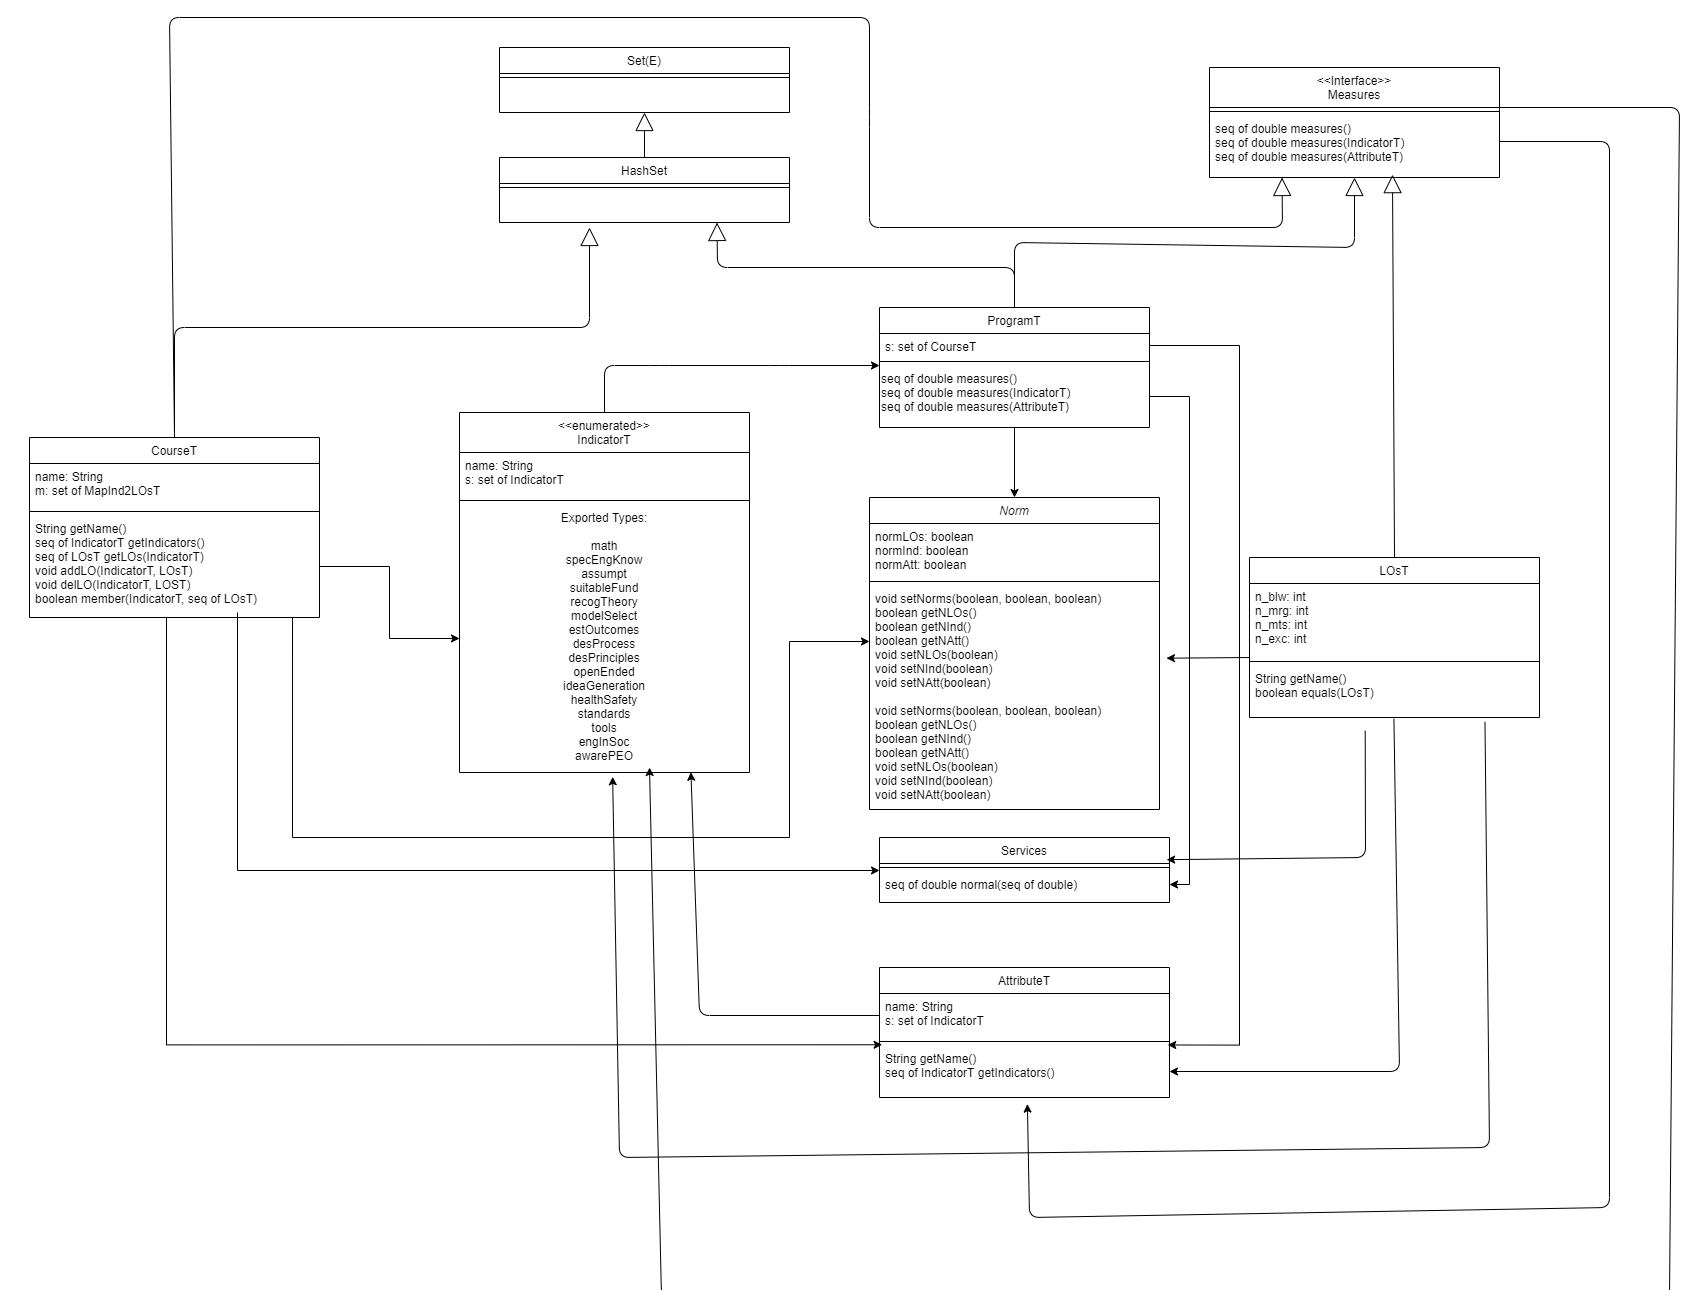
\includegraphics[width=0.6\textwidth]{A3.png}\\
  
	\item Draw a control flow graph for the convex hull algorithm.

\begin{center}
  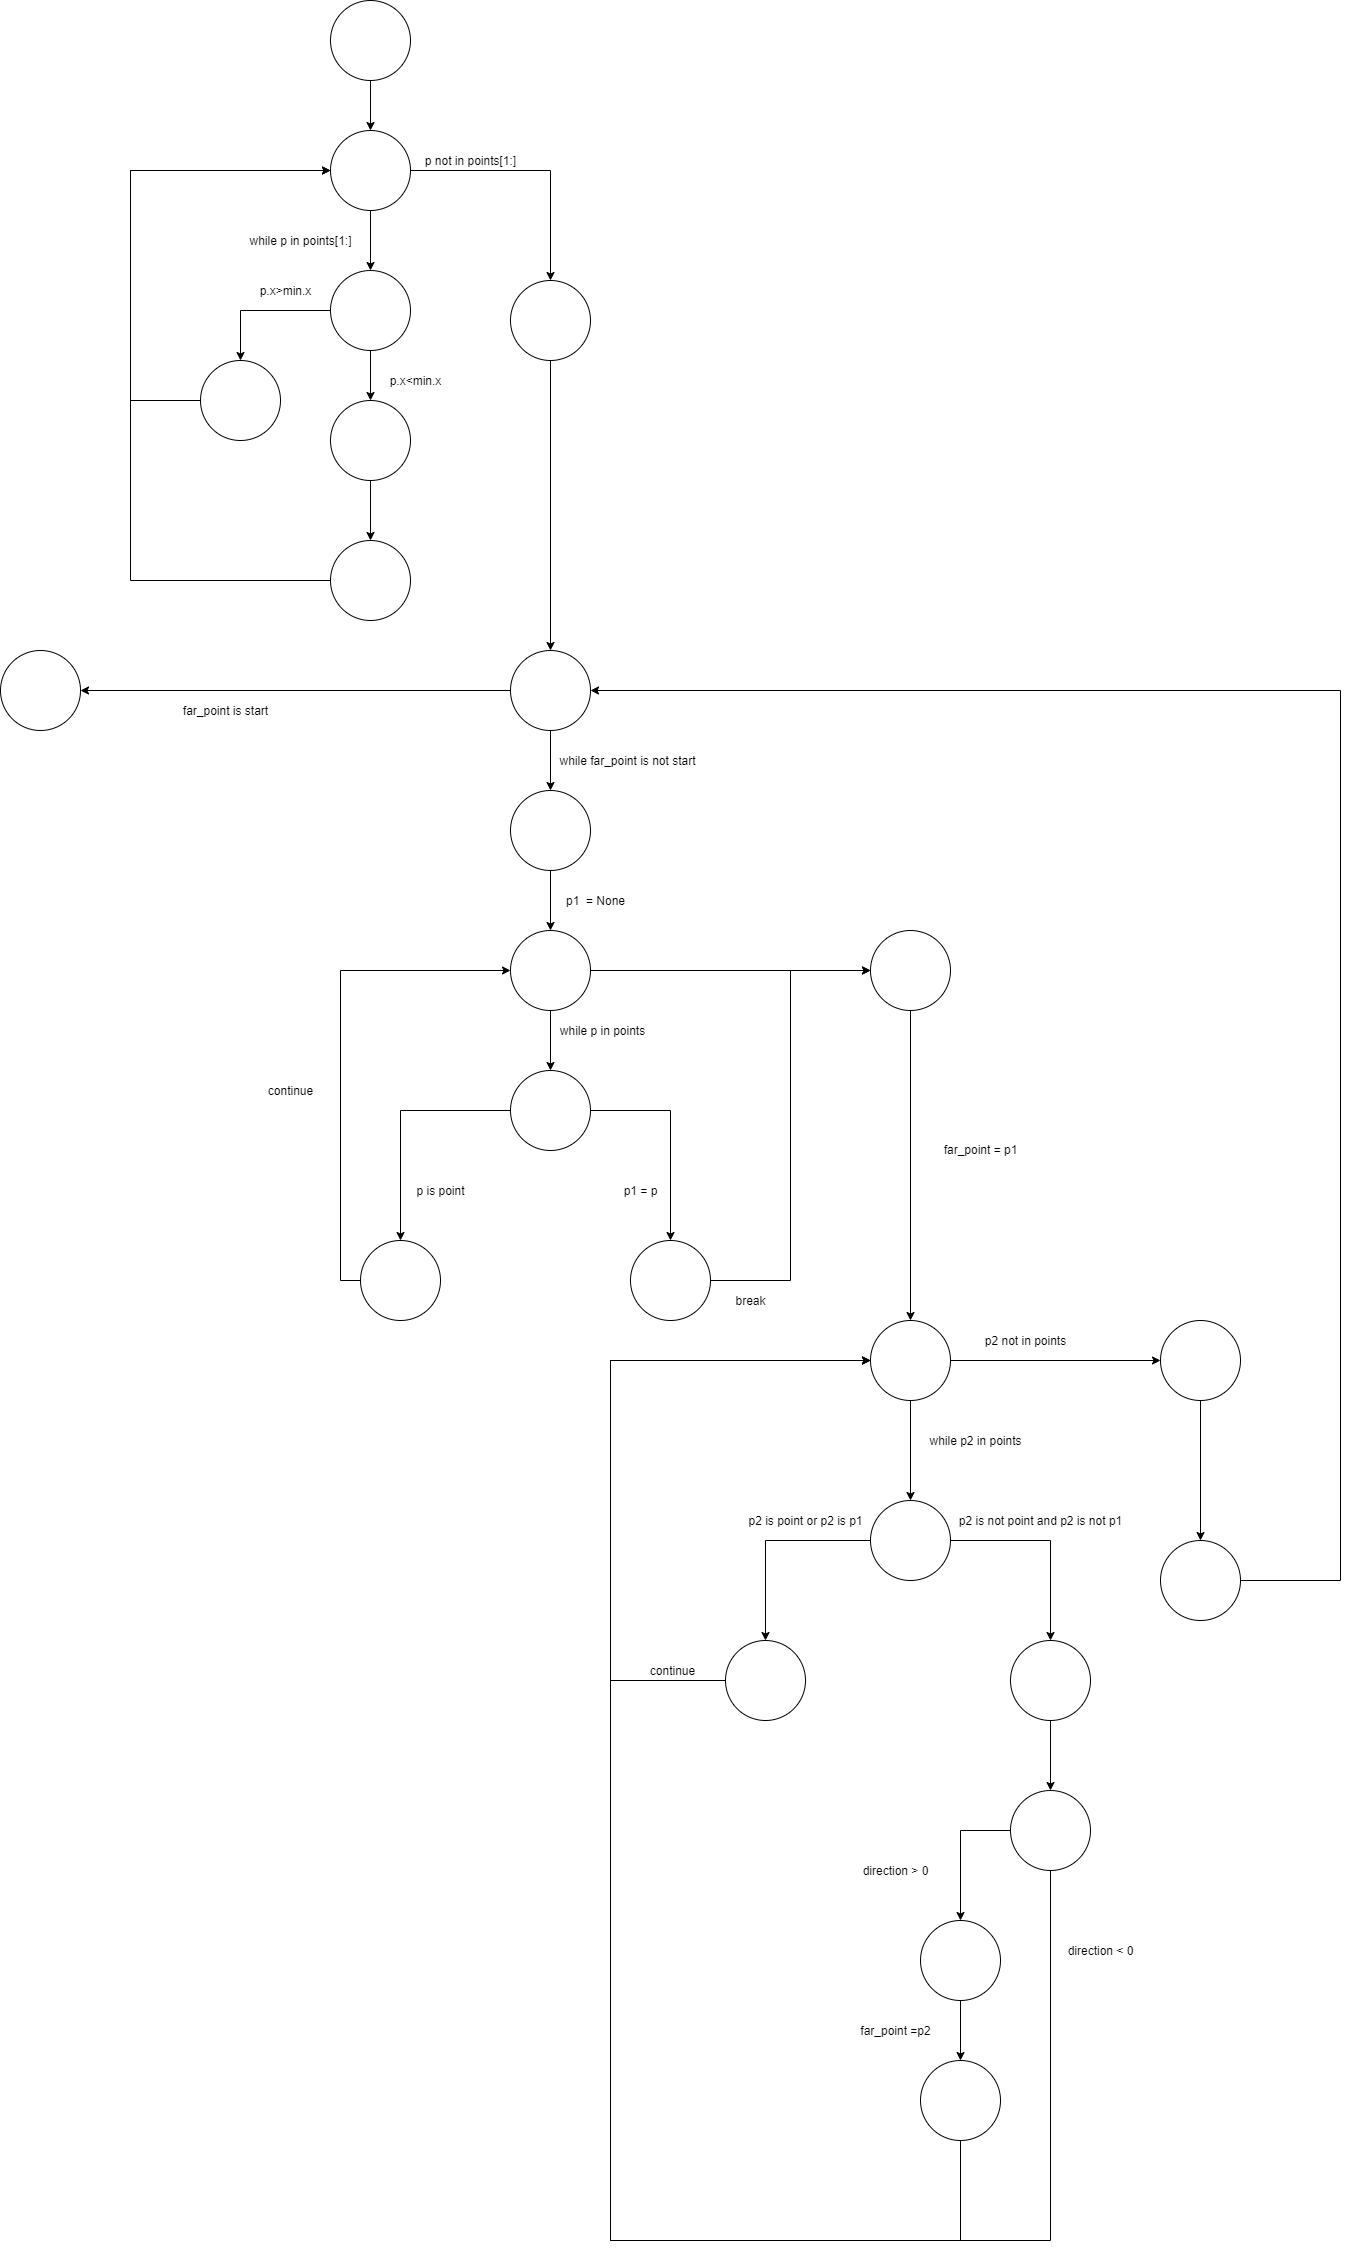
\includegraphics[width=0.6\textwidth]{ControlFlow.png}\\
  Based on \verb|compute_hull()| in https://startupnextdoor.com/computing-convex-hull-in-python/.
\end{center}
\end{enumerate}



\section*{Critique of Specification}

Consistency is shown in the specification through the order of parameters and the consistant naming convention among each module. The ordering of each parameter is the same for each method. For instance, the parameter \verb|row| would always go before \verb|col|. This is almost a standard when we use these two naming conventions together.  In addition, the names of each parameter is consistant through each module. Anything named boardT would mean a \verb|BoardT| object. Similarly, a state variable with the name \verb|board| is the two dimentional array of tiles that is found within a \verb|BoardT| object. Overall, the specification is consistant.

Essentiality omits any unecessary features and ensures that the service is only offered once. The specification is essential as each method does not have a similar method that provides the same service. For instance, within \verb|Move|, \verb|mergeLeft| cannot be achieved through \verb|mergeRight| or any other methods withn \verb|Move|. In \verb|BoardT|, one can argue that getting the value of each tile within a row can be achieved by getting the board through \verb|getBoard| and then looping through each tile within the row. However, this would be a painful and tedious process to repeat each time. Thus, having a method that returns an integer of values in a specific row, would be deemed more convenient. Overall, the access programs within the specification are essential. 


Generality means open endness and anticipating changes. Due to the separation of concerns (i.e. having multiple logical modules instead of one), implementing changes to the specification and code would be easier. For instance, having the controls separate from the board would allow one to reuse the board module not just in ASCII graphics, but also with GUI implementation. In addition, using a data structure such as an array would allow the programmer to easily make changes in the future as all the data is stored in a single space. However, there are other ways to make a specification more general, but was not achieved here in this specification. For instance, instead of putting $4$ when looping through the board, the design would be more general by replacing that with a variable such as $size$. $Size$ can modified easily if one wants to change the size of the board. In addition, a generic module is possible to implement for certain types such as integers, but is awkward if implemented with a string, for instance. 

Minimality means that each access program only does one thing. I have tried to design a specification that is minimal. For instance, \verb|checkWin| within \verb|BoardT| only checks if there is a tile with the value of 2048. After checking, it just returns a boolean and does not, for instance, sets the message to the winning message through \verb|setWinMessage|. Almost all of the access programs are minimal. One that I could not make minimal was the local function \verb|combine| in \verb|Move|.  \verb|combine| merges tiles of the same value together. Within \verb|combine|, it is more convenient if the scores are updated right when the tiles are merged. In a sense, it made the implementation of the specification easier, however, minimality was lost in the process.

Cohesion is an internal property of the module. The components of the modules are grouped together through logical reasoning and not by chance. The specification consists of modules that concern the board, the interface, and the control. Through MVC design pattern, it provides separation of concerns, allowing the modules to be separated appropriately and focus on one related goal per module. Furthermore, there is high cohesion among the components of each module as the methods within the module are related to each other and logically belong in their respective module. For instance, all methods within \verb|TileT| focuses on setting or getting a tile within the board. On the other hand, \verb|BoardT| methods focus on changing and updating the state of the board game. For instance, checking for win or lose make sense to be in \verb|BoardT| and not \verb|TileT| as winning and losing concerns the state of the board and not just the tiles within the board. Thus, the high cohesion is shown through the strong relationship of the components within the module and the separation of concerns of each module.

Information hiding is characterized by the secrets that are hidden from the clients. Through the MVC design pattern, information hiding is already seen as there is a specific module for the user interface. The user interface is what the client would see and interact with. Thus, the backend logic behind how the game works is hidden and encapsulated through \verb|BoardT|. In addition, small design details such as private variables, prevents unanticipated changes to be made within the code and ensures that it cannot be directly accessed through other modules. Therefore, information hiding is seen in the specification through MVC design pattern, separation of concerns and encapsulation.

\end{document}